\section{Einrichtung des ADS-Workspaces}

    \subsection{Auswahl der Technologie und Erstellung des Substrat-Files}
    Bevor wir in ADS die Leitungen Simulieren können, muss das Substrat file definiert werden.
    Hier lässt sich die dicke der Kupferleitung sowie von dem Dielektrikum FR4 wählen.
        \begin{itemize}
            \item FR4    : 1mm
            \item Kupfer : 35\textmu m
        \end{itemize}
        \begin{figure}[H]
            \centering
            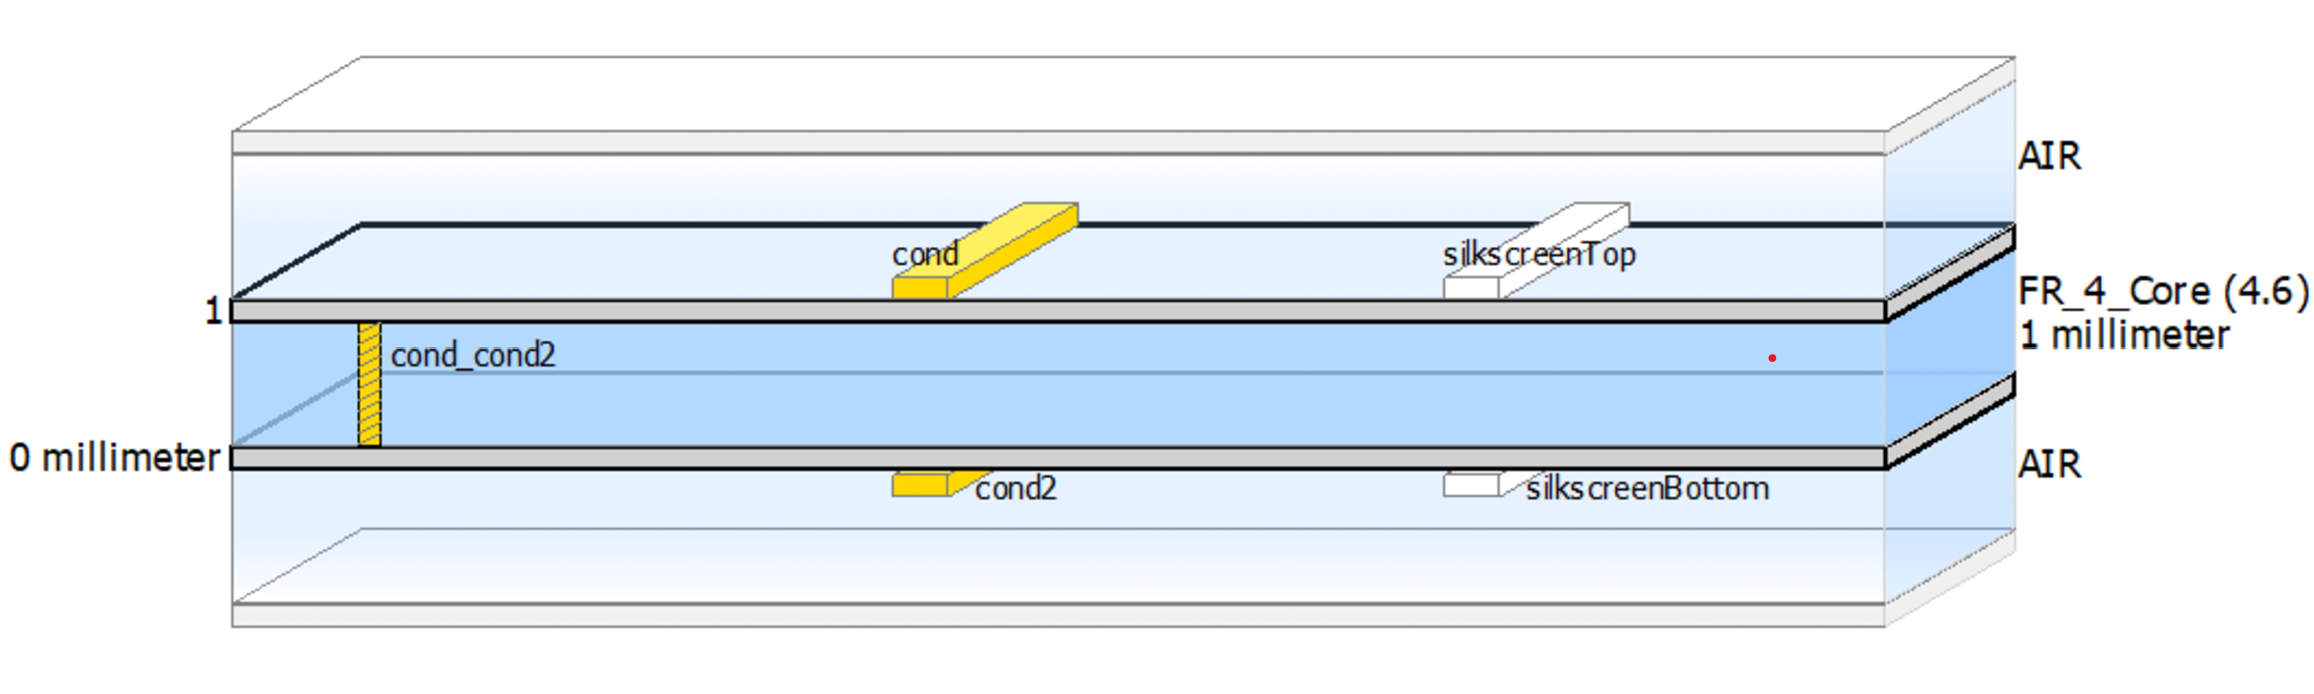
\includegraphics[width=0.9\textwidth]{Pictures/substratFile.png}
            \caption{Substratfile}
        \end{figure}

    \subsection{Nutzung des Controlled Impedance Line Designers}

\section{Leitungsdimensionierung}
    \subsection{\texorpdfstring{Berechnung der Leitungsbreite ($Z_0 = 50~\Omega$)}{Berechnung der Leitungsbreite (Z0 = 50 Ohm)}}
    Nun wird die Leitungsbreite einer Microstrip Leitung mit der Wellenimpedanz $Z_0 = 50~\Omega$ berechnet.
    Dazu verwenden wir die Formeln, die uns auf der Webseite von MIcrowases101 Kapitel Microstrip zur
    Verfügung gestellt werden. Durch eine grobe Abmessunge sieht man das folgende Beziehung gilt \\
    \[
    \frac{w}{h} < 1
    \]


    \subsection{Verifizierung der Berechneten Leitungsbreite}
    Nun wird die Leitungsbreite mithilfe des Controlled Impedance Line Designers Simuliert.
    Ziel ist es die $Z_0 = 50~\Omega$ zu erreichen durch sweepen der Leitungsbreite
    \begin{figure}[H]
        \centering
        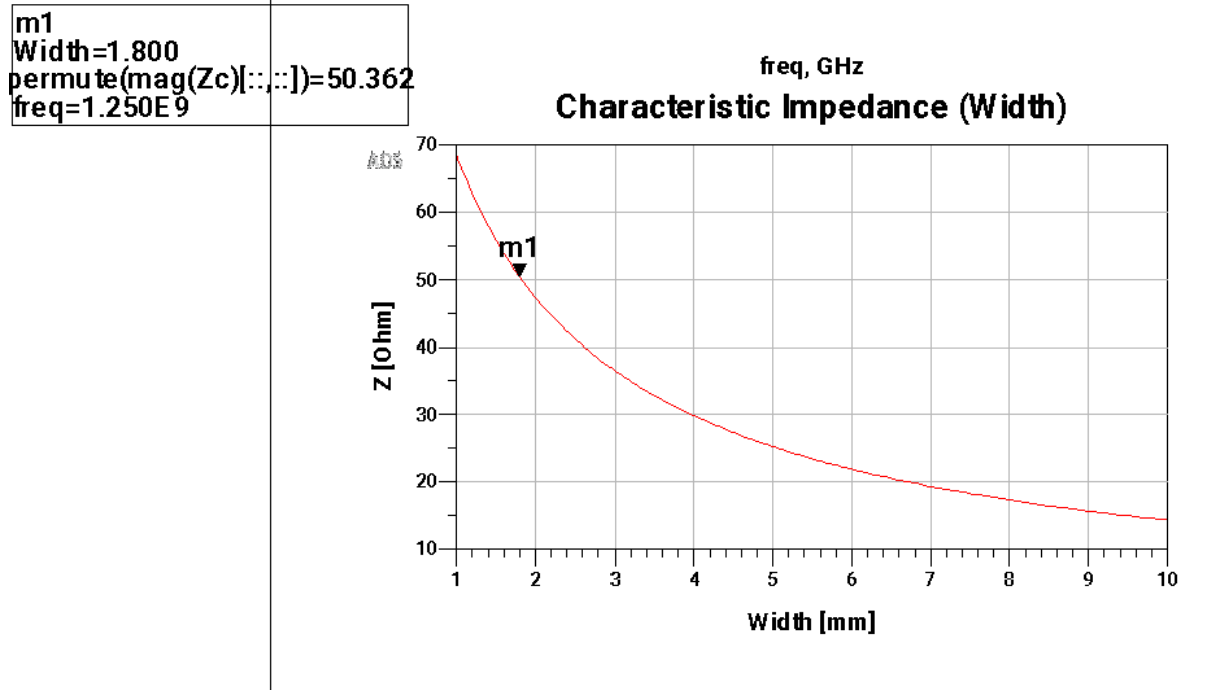
\includegraphics[width=0.8\textwidth]{Pictures/LeitungsbreitenSweep.png}
        \caption{Wellenimpedanz in abhängigkeit von der Leitungsbreite}
    \end{figure}
    Wie schon numerisch bestimmt kommen wir mitn der Leiterbreite $w=1.8mm$ der Wellenimpdanz $Z_0 = 50~\Omega$
    am nähesten. Würde man noch genauer sweepen, wird man festellen dass die Optimale Leiterbreite irgendwo zwischen
    $1.8mm$ und $1.9mm$ liegt.

    \subsection{Charakteristische Länge der Koppelleitungen}
    \subsection{Bestimmung der Filterordnung}

\section{Aufbau des Coupled-Line-Filters im Schematic}

\section{Simulation und Optimierung}
    \subsection{Vergleich mit Messdaten}

\section{Knick zur Optimierung des Aspektverhältnisses}

\section{Anpassung im Schematic und Re-Simulation}

\section{Auswirkungen auf die S-Parameter}
